\documentclass{standalone}

\usepackage{tikz}
\usetikzlibrary{circuits.logic.US}
\usetikzlibrary{positioning}

\begin{document}
	
	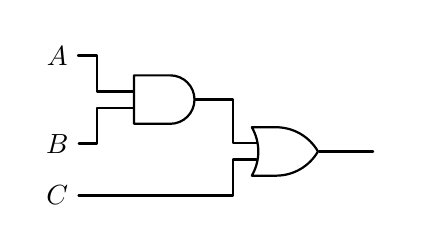
\begin{tikzpicture}[circuit logic US,
	line width=0.8pt,line cap=round,line join=round]
	
	\matrix[column sep=7mm]
	{
        \node (A) {$A$}; &     & & \\
		                 & \node [and gate] (and1) {};      & & \\
        \node (B) {$B$}; &     & \node [or gate,yshift=-1mm] (or1) {}; & \node[yshift=-1mm] (out) {};\\
        \node (C) {$C$}; &     & & \\
	};
	
	\draw 
	
	% AND gate inputs
	(A) -- ++(right:5mm) |- (and1.input 1)
	(B) -- ++(right:5mm) |- (and1.input 2)
	
	% OR gate inputs
	(or1.input 1) -- ++(left:3mm) |- (and1.output)
	(or1.input 2) -- ++(left:3mm) |- (C)
	
	% Output
	(or1.output) -- (out);
	\end{tikzpicture}
	
\end{document}